\section{Weak Learnability}

\begin{frame}{What exactly is a weak learner?}
    \textbf{Remember, that a strong PAC learner for a class $\mathcal{H}$...} \pause
    \begin{itemize}
        \item ...if it is presented with $m > m_\mathcal{H}(\epsilon, \delta)$ examples \pause
        \item ...has to find a hypothesis $h \in \mathcal{H}$ \pause
        \item ...such that $L_{(\mathcal{D}, f)}(h) < \epsilon$ for every $D$ and $f$ with confidence $1 - \delta$ (if RA holds) \pause
    \end{itemize}
    \vspace{0.5cm}
    \centering
    \fbox{\textbf{In weak learning, we only want the error to be less than 50\%.}}
\end{frame}

\begin{frame}{Weak learning definition}
    \textbf{An algorithm A is a $\gamma$-weak-learner for a class $\mathcal{H}$, if...} \pause
    \begin{itemize}
        \item ...for every $\delta \in (0, 1)$ there exists a threshold 
            $m_{\mathcal{H}}(\delta) \in \mathbb{N}$, such that \pause
        \item ...if trained on at least $m > m_{\mathcal{H}}(\delta)$ examples \pause
        \item ...it will find a hypothesis $h$, such that \pause
        \item ...$L_{(\mathcal{D}, f)}(h) < \frac{1}{2} - \gamma$
            with confidence $1 - \delta$ \pause
        \item ...for every labeling function $f$ and every distribution $\mathcal{D}$
            (if RA holds) \pause
    \end{itemize}
    \textbf{...but how does this help us?}
\end{frame}

\begin{frame}{Why we care about weak learning}
    \begin{itemize}
        \item We already know that implementing ERM for strong learners can be
            computationally hard \pause
        \item Weak learners don't have to be that accurate (only better than 50\%) \pause
        \item Maybe we can find weak learners that can be implemented efficiently \pause
        \item ...and then use boosting to still end up with a strong learner \pause
    \end{itemize}
    \textbf{Lets look at an example (Decision Stumps)}
\end{frame}

\begin{frame}{Spam detection with decision stumps}
    \begin{figure}
        \centering
        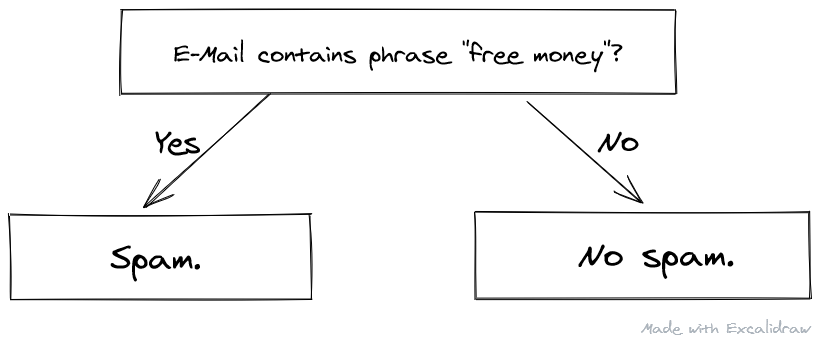
\includegraphics[width=\textwidth]{img/spam_classifier.png}
        \caption{This is a Decision Stump.}
    \end{figure}
\end{frame}

\begin{frame}{ERM for decision stumps is efficient}
    \begin{itemize}
        \item Decision Stumps partition the instance space $\mathcal{X}$
            along a single dimension \pause
        \item This is the hypothesis class: \pause
    \begin{equation*}
        \mathcal{H}_{DS} = \{ \mathbf{x} \mapsto \text{sign}\left( \theta - x_i \right) \cdot b: \ 
        \theta \in \mathbb{R}, i \in \left[ d \right], b \in \{ \pm 1 \} \}
    \end{equation*} \pause
        \item ERM has to find the best threshold $\theta$ and the best
            dimension $i \in [d]$ such that
            the training error is minimized:\footnote{$D_i$ are sample weights} \pause
    \end{itemize}
    \begin{equation*}
        \min_{j \in \left[ d \right]} \  \min_{\theta \in \mathbb{R}} \ 
        \left( \sum_{i: y_i=1}^m D_i \mathds{1}_{\left[ x_{i, j} > \theta \right]} + 
            \sum_{i: y_i=-1}^m D_i \mathds{1}_{\left[ x_{i, j} \leq \theta \right]} \right)
    \end{equation*} \pause
    \centering
    \fbox{\textbf{This can be solved in $\mathcal{O}(dm)$!}}
\end{frame}

\begin{frame}{What we learned so far}
    \begin{itemize}
        \item What is a weak learner? \pause
        \begin{itemize}
            \item[$\rightarrow$] An algorithm that finds a hypothesis that
                performs better than random
        \end{itemize} \pause
        \item What are decision stumps? \pause
        \begin{itemize}
            \item[$\rightarrow$] A simple hypothesis class where ERM is efficient.
                Decision stumps partition the feature space along a single dimension.
        \end{itemize} \pause
        \item What is the idea behind boosting? \pause
        \begin{itemize}
            \item[$\rightarrow$] Use an efficient weak learner to create weak hypotheses.
                Combine them to get a strong hypothesis.
        \end{itemize} \pause
    \end{itemize}
    \textbf{But how to do that? The AdaBoost algorithm will tell us...}
\end{frame}